% CVPR 2025 Paper Template; see https://github.com/cvpr-org/author-kit

\documentclass[10pt,twocolumn,letterpaper]{article}

%%%%%%%%% PAPER TYPE  - PLEASE UPDATE FOR FINAL VERSION
%\usepackage[review]{cvpr}      % To produce the REVIEW version
\usepackage{cvpr}

% Import additional packages in the preamble file, before hyperref
%\input{preamble}

% It is strongly recommended to use hyperref, especially for the review version.
% hyperref with option pagebackref eases the reviewers' job.
% Please disable hyperref *only* if you encounter grave issues, 
% e.g. with the file validation for the camera-ready version.
%
% If you comment hyperref and then uncomment it, you should delete *.aux before re-running LaTeX.
% (Or just hit 'q' on the first LaTeX run, let it finish, and you should be clear).
\definecolor{cvprblue}{rgb}{0.21,0.49,0.74}
\usepackage[pagebackref,breaklinks,colorlinks,allcolors=cvprblue]{hyperref}

\usepackage{listings}
\usepackage{tabularx}

%%%%%%%%% PAPER ID  - PLEASE UPDATE
\def\paperID{*****} % *** Enter the Paper ID here
\def\confName{CVPR}
\def\confYear{2025}

%%%%%%%%% TITLE - PLEASE UPDATE
\title{Diffusion Models for Dynamic Video Synthesis with Image and Text Prompts Guidance}

%%%%%%%%% AUTHORS - PLEASE UPDATE
\author{
First Author\\LeHao Ling\\{\tt\small firstauthor@i1.org}\\45\%
\and
Second Author\\YuXuan Huang\\{\tt\small cxlhyx1297767084@gmail.com}\\35\%
\and
Third Author\\JianLin Luo\\{\tt\small firstauthor@i1.org}\\20\%
\\
\\Institution\\School of Artificial Intelligence, South China Normal University
\\Institution address\\Foshan, 528225, China
\\\hyperref[https://github.com/cxlhyx/DL-CLASS-PROJECT]{\textbf{https://github.com/cxlhyx/DL-CLASS-PROJECT}}
% For a paper whose authors are all at the same institution,
% omit the following lines up until the closing ``}''.
% Additional authors and addresses can be added with ``\and'',
% just like the second author.
% To save space, use either the email address or home page, not both
}

\begin{document}
    \maketitle
    \begin{abstract}
    This article introduces a method for generating text, images, and videos by integrating image prompts and Large Language Models (LLMs) to address the challenges of appearance generation and spatiotemporal consistency. We propose a method of using LLM to refine prompts, decomposing abstract prompts into concrete prompts to enhance dynamic understanding. In addition, we have improved the global dynamics and content movement in generated videos by combining image guidance with position encoding and coarse to fine fusion strategies. A novel text image video dataset based on the WebVid-10M dataset is constructed for training and evaluation, and its performance is evaluated using the CLIP scoring metric. Our contributions include refining video summarization prompts, image-guided video generation, and dataset construction, significantly improving the quality of video generation. This work is of great significance for content creation, gaming, and film production, providing a promising direction for future research on text to video generation. Our work is already underway \hyperref[https://github.com/cxlhyx/DL-CLASS-PROJECT]{\textbf{https://github.com/cxlhyx/DL-CLASS-PROJECT}} upload.
\end{abstract}    
    \section{Introduction}
\label{sec:Introduction}

Text-to-video models has attracted widespread attention as a type of deep learning model\cite{blattmann2023align,esser2023structure}, it generates videos by taking text descriptions as inputs. A video can provide more informative, attractive, and immersive visual content, which can benefit novel content creation, gaming, and movie production \cite{he2022latent}. Therefore, it is very necessary to study how to better use text to generate videos.\\
\indent Most existing studies start with simple text prompts only, such as Free-Bloom \cite{huang2024free}, Text2Video-Zero \cite{li2023amt}, both of them are zero-shot text-to-video Generators. In this way, there are some problems, we point out two obvious issues. One is models cannot generate the desired appearance, the other is space-time consistency issues.\\
\indent In order to solve the first problem, an intuitive method is to use images as references, called image prompts. Image prompts complement text prompts and enrich the details that are difficult to describe with text prompts. There are two main types of attempts at image prompts. One is to use a few-sample reference images to fine-tune some parameters \cite{choi2023custom}, and the other is to embed images into the video model and the inference is tuning-free \cite{chen2023disenbooth}. Jiang explore the task of video generation using image prompts without finetuning at inference time, and proposed VideoBooth \cite{jiang2024videobooth}, which generates consistent videos containing the desired subjects. However, during our experiments, we found that the videos generated by VideoBooth lacked global dynamics and the content was difficult to move.\\
\indent Free-Bloom generate high-quality, space-time consistent, and semantically aligned videos by harnessing large language models (LLMs) as the director, while pretrained image diffusion models as the frame animator. Referring to Free Bloom and VideoBooth, we propose video summary prompts and image prompts to video generation with adding DSL to guide video generation and using dynamic weights for conditional fusion.\\
\indent We conducted our method on the WebVid-10M dataset, which is a classic video dataset consisting of 10M video clips with a duration mostly within 30s. Each video is accompanied by a corresponding textual description and has a dataset format similar to OpenVid-10M. Overall, it contains information such as the video file name, text description, frame rate, duration, etc.\\
\indent In summary, our contributions can be summarized as:\\
\indent 1) Video Summary Prompt Refinement: We enhance video generation by leveraging LLMs to decompose abstract prompts into multiple concrete ones, which are encoded via CLIP to guide frame-by-frame generation, improving dynamics and abstract understanding.\\
\indent 2) Image-Guided Video Generation: Introducing position encoding, incorporating image guidance alongside text prompts and adopting a coarse-to-fine fusion strategy inspired by VideoBooth.\\
\indent 3) Data augmentation: Constructed a dataset for image guided video generation.\\
\indent This article will start from these aspects: Section 1 is the introduction, Section 2 is the related work, Section 3 we provide a detailed description of our method, Section 4 we conducted our method on the WebVid-10M dataset, Section 5 is the discussion about our method, Section 6 we summarize our article.
    \section{Related Works}
\label{sec:Related Works}
In this section, we will elaborate on the following aspects, diffusion models, text-to-video models, Text-to-Video Models with Image prompt.

\subsection{Diffusion Models}
Diffusion models are a class of likelihood-based generative models that have shown remarkable progress in image generating tasks \cite{rombach2022high,ruiz2023dreambooth}. The several models mentioned in the introduction are all based on diffusion models as baselines, additionally, diffusion models have a thriving research and application ecosystem, including multiple works \cite{mou2024t2i} as well as emerging open-source communities and libraries \cite{wang2023zero} with frameworks and plugins.\\
\indent The core of the diffusion model lies in two key steps: the forward diffusion process and the reverse generation process. The forward process gradually maps the data to a Gaussian distribution by adding noise, while the reverse process gradually denoises to restore the data through a parameterized network (such as U-Net).\\
\indent In the development of diffusion models, Denoising Diffusion Probabilistic Models (DDPM) is one of the earliest widely studied frameworks. DDPM trains the denoising process at each step by optimizing an objective function based on a variational lower bound. This method generates high-quality samples, but the computational cost is high, especially in the inference stage, which requires a large number of time steps (such as hundreds of steps) to complete denoising. In order to solve this problem, Denoising Diffusion Implicit Models (DDIM) proposes an improved method to reduce the number of generation steps, and significantly improves the generation speed by switching to a deterministic reverse process.\\
\indent Another important development in diffusion models is the combination of large-scale data and computing power for pre-training. In recent years, models such as Imagen and Stable Diffusion have demonstrated the power of diffusion models in text-to-image generation tasks. These models enable the generated images to be accurately matched to complex textual descriptions by combining a diffusion process with multi-modal embeddings of large language models such as Transformer. At the same time, the open source of these models promotes the practical application of diffusion models in art creation, game design and other fields.\\
\indent The applications of diffusion models are not limited to image generation. In video generation, diffusion models are used to generate consecutive video frames by extending the spatial dimension to the temporal dimension. Although diffusion models are powerful, they also face some challenges, such as spatiotemporal consistency issues. Therefore, how to further optimize the generation process, improve training efficiency and expand multi-modal capabilities is still a hot topic in current research.

\subsection{Text-to-Video Models}
Early explorations of text to video models \cite{hong2022cogvideo,villegas2022phenaki} were based on the idea of VKVAE, while recently, the emergence of diffusion models \cite{ho2020denoising,rombach2022high} has driven further research in this field \cite{an2023latent}. The diffusion based text to video model demonstrates stronger capabilities, such as Video Diffusion Models (VDM). These models improve temporal consistency while ensuring video frame quality by extending the diffusion process on the timeline. Imagen Video \cite{an2023latent} is based on Google's Imagen framework and uses a large-scale text to image generation model as a foundation to gradually generate high-quality videos by increasing the temporal dimension. Similarly, Meta's Make-a-Video \cite{singer2022make} uses a small amount of video data to extend the existing image generation model for temporal modeling, demonstrating the ability to generate high fidelity videos in different scenarios. These models typically rely on large-scale language visual pre training data, as well as efficient sampling and multi-scale generation strategies.\\
\indent The open-source development of Stable Diffusion has driven community research on Wensheng video models, with some projects combining Stable Diffusion with temporal modeling components such as Transformer or LSTM to generate high-resolution and frame consistent videos. In addition, research extending to the generation of long videos has gradually received attention, such as generating longer videos with better continuity through segmented generation and concatenation.\\
\indent In terms of technology, spcae-time consistency is a key direction. Some works enhance consistency by modeling the latent variable space over time (such as using CLIP or other visual language models to supervise each frame generation). In addition, domain specific fine-tuning based on real video data has been proven to effectively improve the diversity and reliability of model generation.

\subsection{Text-to-Video Models with Image prompt}
The image-based video model is of great significance in generative artificial intelligence. This type of model uses input text and static images as starting points to generate dynamic time series, providing creators with a natural transition from static to dynamic content. Compared to completely text-based generation, image prompts can provide more initial visual information, enhancing the model's understanding of scene layout, subject features, and details. This method is widely used in fields such as virtual reality, advertising creation, and video editing.\\
\indent Early research was typically based on GAN (Generative Adversarial Network) architectures, such as MoCoGAN \cite{tulyakov2018mocogan} and TGAN, which extended static images into continuous videos by decoupling image content and motion features. However, these methods face challenges in generating inter frame consistency and high-quality details, especially for the generation of long-term videos. With the development of VAE (Variational Autoencoder) and VKVAE (Vector Quantization Variational Autoencoder) technologies, latent variable based generative models provide new ideas for image to video generation. For example, by modeling the temporal sequence of latent variables in images, continuous video frames that conform to dynamic logic can be generated.\\
\indent In recent years, the rise of diffusion models has further promoted the development of image-based video models. The gradual denoising process of the diffusion model is very suitable for dealing with inter frame temporal consistency issues. For example, models such as Imagen Video \cite{ho2022imagen} and Make-A-Video \cite{singer2022make} embed static images into the generation process of diffusion models to generate high-quality dynamic videos while preserving input image details. In addition, these models are often combined with powerful multimodal pre training models (such as CLIP or large language models) to enable the generated videos to match auxiliary text descriptions, thereby providing higher semantic control.\\
\indent VideoBooth \cite{jiang2024videobooth} is also a type of image-based generative video model, which consists of two modules: a coarse embedding module through an image encoder and a fine embedding module through attention injection. The image encoder provides rough embedding of image prompts to refine the attention injection module. These two modules work together to train in a coarse to fine manner. In this article, we will use VideoBooth as a baseline for further research.
    \section{Method}
In this section, we will introduce our method.

\begin{figure*}
    \label{main_framework}
    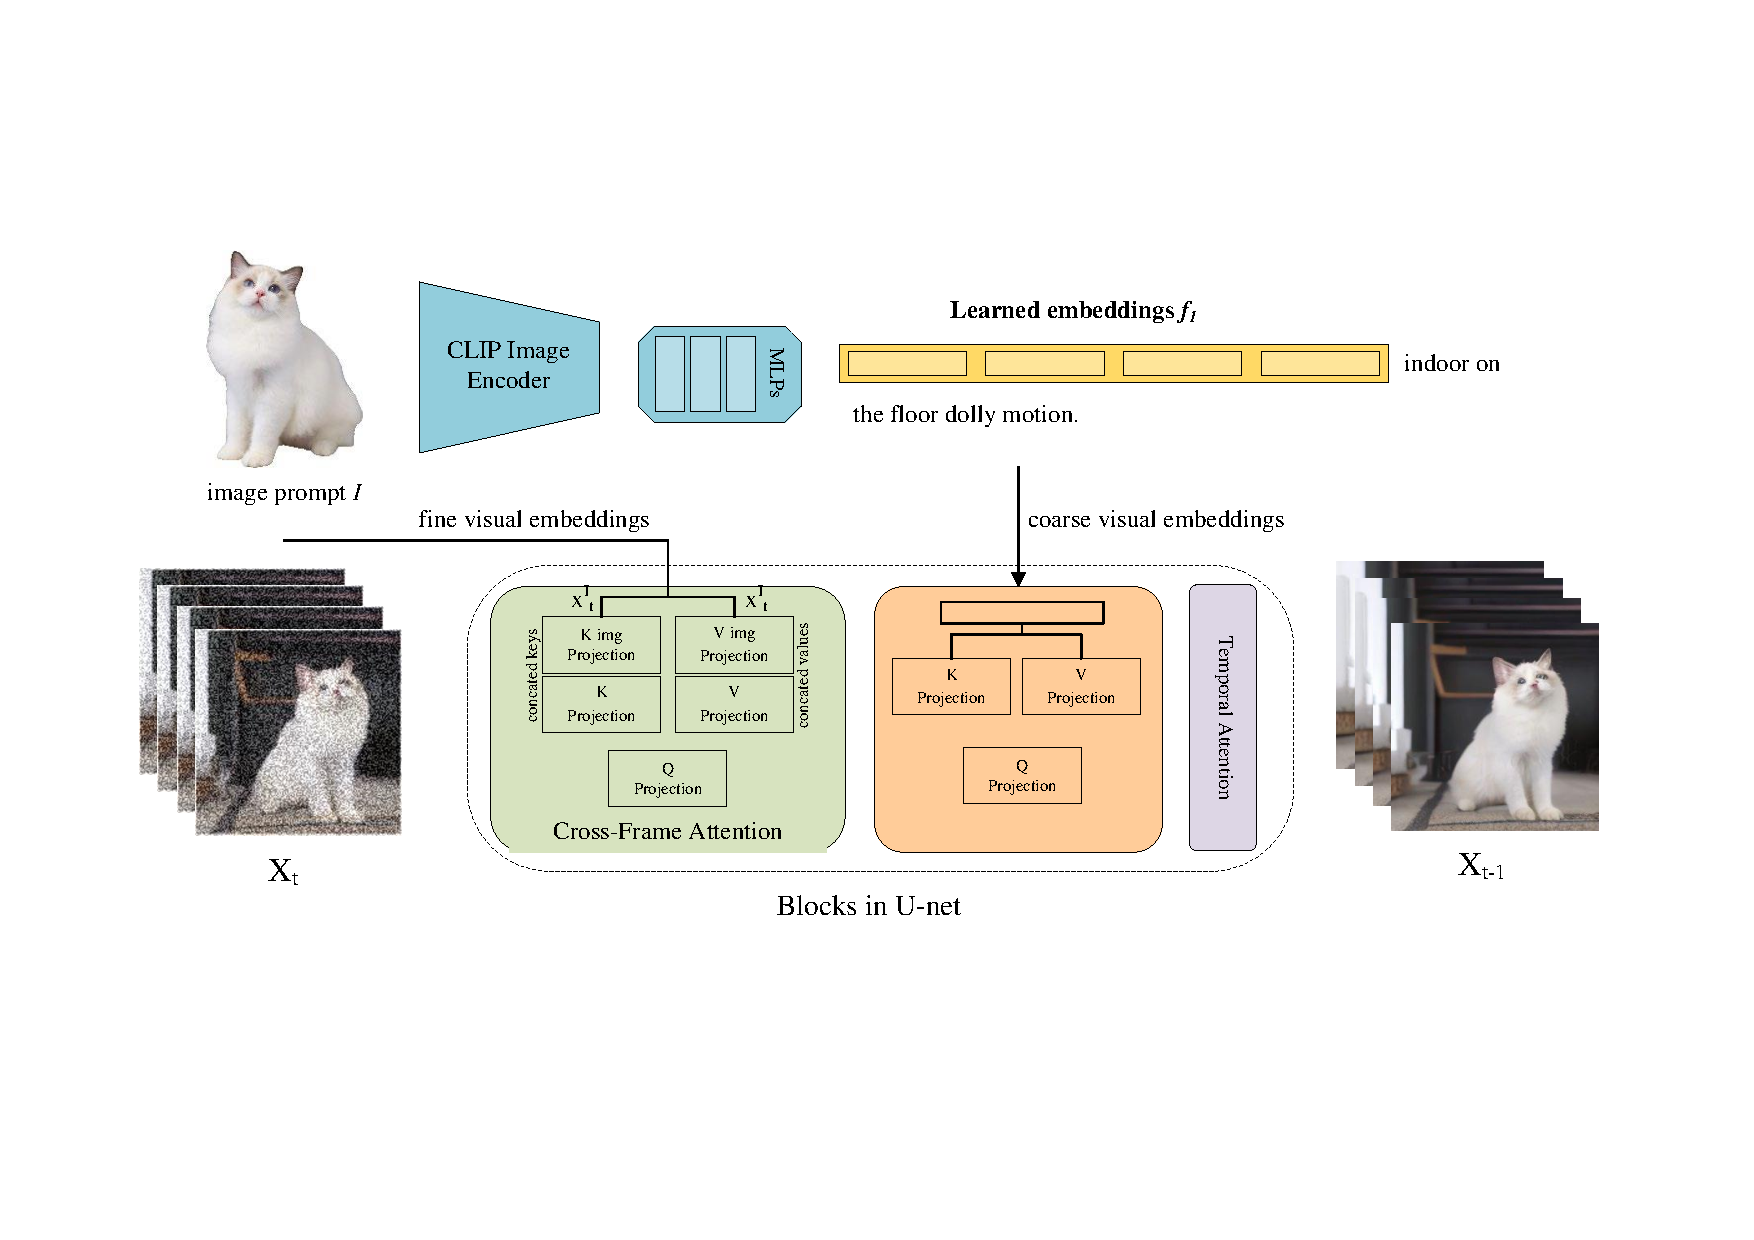
\includegraphics[width=\linewidth]{fig/main_framework.pdf}
    \caption{main\_framework}
\end{figure*}

Our proposed method aims at generating videos from an image prompt I and a text prompt T. As shown in \hyperref[main_framework]{Fig 1}, we use the image prompt specifies the appearance of the subject, which is fed into in two levels. First, we fed into a pretrained CLIP Image encoder to extract visual features. The encoder is composed of several MLP layers and is trained to map visual features into the space of text embeddings. After we obtain the embedding $f_I$, we insert them into text embedding, which is extracted by feeding text prompt $T$ into CLIP text encoder. In order to refine the details, we inject image prompt $I$ into the cross-frame attention module in the pretrained video diffusion model. Specifically, we incorporate the latent representation $x_t^I$ of the image prompt $I$ into the cross-frame attention mechanism. This approach integrates multi-scale visual details along with spatial information into the computation of attention maps, enhancing the preservation of visual characteristics. The image prompt is utilized in two complementary ways, operating in a coarse-to-fine manner: the encoder supplies coarse visual embeddings of the image prompt, while the attention injection introduces fine-grained visual embeddings.

\subsection{Coarse Visual Embeddings via Image Encoder}
Given an image prompt \(I\) and a text prompt \(T\), the generated video should align with both visual and textual elements. Inspired by previous image-based customization methods, we propose to encode the visual information of image prompts using an image encoder. The image prompt provides the visual characteristics of the desired subject in the video, while the text prompt contributes complementary information. The extracted visual embeddings are combined with text embeddings to form the final embeddings used in the cross-attention module.

Specifically, we utilize a pretrained CLIP image encoder to extract the visual features \(f_V\) from the image prompt \(I\). Since there is a discrepancy between CLIP image and text embeddings, \(f_V\) is mapped into the text embedding space using MLP layers \(F(\cdot)\), resulting in the final embedding \(f_I\) for the image prompt:

\[f_V = \text{CLIP}_I(I), \quad f_I = F(f_V)\]

The text prompt \(T\) is processed by the CLIP text encoder to extract text embeddings \(f_T\):

\[f_T = [f_T^0, f_T^1, \dots, f_T^k, \dots]\]

To integrate \(f_I\) and \(f_T\) for diffusion model conditioning, we replace the word embedding of the target subject in the text prompt with \(f_I\), resulting in the final text condition \(c_T\):

\[c_T = [f_T^0, f_T^1, \dots, f_T^{k-1}, f_I, f_T^{k+n}, \dots]\]

During training, the parameters of the CLIP image encoder are fixed, and the MLP layers are optimized. Additionally, we finetune the \(K\) and \(V\) projection layers in the cross-attention module to accommodate the composed embeddings \(c_T\).

\subsection{Fine Visual Embeddings via Attention Injection}
While the image encoder provides coarse visual embeddings, its high-level flattened representation may result in the loss of fine-grained visual details. To address this, we propose injecting the image prompt into the cross-frame attention module of the text-to-video model, allowing the model to directly incorporate detailed visual cues from the image prompt into the synthesized frames.

The image prompt is first passed through the VAE of Stable Diffusion to obtain its latent representation \(x_I\). Since video generation starts from noise, the latent representation needs to align with the intermediate states by adding noise:

\[x_I^t = \sqrt{\alpha_t}x_I^0 + \sqrt{1-\alpha_t}\epsilon\]

In cross-frame attention, we first update the values \(V_0\) of the first frame using the keys and values derived from the image prompt:

\[V_0^{\text{new}} = \text{softmax}\left(\frac{KQ_0^T}{\sqrt{d}}\right) \cdot V,\]
\[\quad K = [K_I, K_0], \quad V = [V_I, V_0]\]

Subsequently, the updated \(V_0^{\text{new}}\) is used to refine the remaining frames:

\[V_i^{\text{new}} = \text{softmax}\left(\frac{KQ_i^T}{\sqrt{d}}\right) \cdot V,\]
\[\quad K = [K_0, K_{i-1}], \quad V = [V_0^{\text{new}}, V_{i-1}]\]

To refine details further, we inject multi-scale latent representations of the image prompt into different cross-frame attention layers, using resolutions corresponding to different stages of the U-Net.

\subsection{Coarse-to-Fine Training Strategy}
The visual details of the image prompt are incorporated into the generated results in two stages: coarse visual embeddings via the image encoder and fine visual embeddings via attention injection. We propose a coarse-to-fine training strategy: first, the image encoder is trained to produce coarse embeddings, and then the attention injection module is trained to refine details.

As demonstrated in the ablation study, training both modules simultaneously causes the attention injection module to dominate, resulting in the image encoder learning ineffective representations. This leads to poor results during inference, as the coarse embeddings lack meaningful information to guide the attention injection module. Therefore, a sequential training strategy is essential to ensure the consistency and detail preservation in the synthesized video frames.

\subsection{Position encoding}
Position encoding is essential in transformer models to provide information about the order or position of input data. In our method, which involves generating videos from image and text prompts, position encoding helps capture both spatial and temporal relationships.

We utilize sine-cosine positional encodings, a common choice due to their ability to represent relative positions effectively. The standard formula is:

\[PE_{pos, 2i} = \sin\left( \frac{pos}{10000^{2i/d_{\text{model}}}} \right)\]\[
PE_{pos, 2i+1} = \cos\left( \frac{pos}{10000^{2i/d_{\text{model}}}} \right)\]

Where:
    \( PE \) is the positional encoding,
    \( pos \) is the position index,
    \( i \) is the dimension index,
    \( d_{\text{model}} \) is the embedding dimension.

For images, we extend this to 2D positions, encoding both width and height coordinates separately. For videos, we include temporal positional encodings to handle the sequence of frames.

In our cross-attention mechanism, position encodings are added to the query, key, and value embeddings to maintain coherence in spatial and temporal data. Additionally, for multi-scale latent representations, we scale the positional encodings to match the feature map sizes at different resolutions.

This approach ensures that our model effectively understands and utilizes the positional information in both spatial and temporal dimensions.

\subsection{LLM text prompt}
Large language models (LLMs) have demonstrated remarkable performance across a wide range of natural language tasks, showcasing their ability to understand and generate human language with remarkable accuracy and creativity. Their proficiency in handling complex linguistic structures and contextual nuances makes them invaluable tools for enhancing the quality of text prompts used in various applications, including image and video generation models. In these models, the text prompt serves as a critical guide, influencing the specificity and coherence of the generated content. The effectiveness of the prompt directly impacts the model's performance, and thus, improving prompt quality is essential for achieving desired outcomes.

Given the advantages of LLMs in generating detailed and contextually rich text, we have designed a prompt template \hyperref[LLM_text_prompt]{Table 1} that leverages their capabilities to refine and enhance the text prompts used in video generation models. This template is specifically crafted to capitalize on the LLM's strengths in understanding semantics and generating diverse descriptions, thereby producing more precise and effective prompts. By doing so, we aim to significantly improve the quality and fidelity of the generated videos, ensuring that they align closely with the intended visual content.

\begin{table}
    \caption{LLM text prompt.}
    \label{LLM_text_prompt}
    \begin{tabularx}{\linewidth}{X}
        \hline
            \ \ \ \ a man is playing guitar.\\
            \\
            \ \ \ \ Change the sentence above to something like this (add some facial changes, even if they are minor. Don't make the sentence too long):\\
            \\
            \ \ \ \ The video features a man standing next to an airplane, engaged in a conversation on his cell phone. he is wearing sunglasses and a black top, and he appears to be talking seriously. The airplane has a green stripe running along its side, and there is a large engine visible behind his. The man seems to be standing near the entrance of the airplane, possibly preparing to board or just having disembarked. The setting suggests that he might be at an airport or a private airfield. The overall atmosphere of the video is professional and focused, with the man's attire and the presence of the airplane indicating a business or travel context.\\
        \hline
    \end{tabularx}
\end{table}
    \section{Experiment}
In this section, we will describe our improvement on dataset and model. In addition, we provide results and indicators about our model.

\subsection{Dataset}
In the text-to-video model generated by image guidance, text and image are two important prompts, which are also the inputs of the model. Nowadays, most video datasets are just text-to-video datasets, lacking the image of the video subject, so such datasets cannot be used as input to train textual video models generated by image guidance. To solve this problem, we construct a text-image-video dataset based on the classic video dataset WebVid-10M. The text-image-video dataset includes videos, their textual descriptions, and the subject's location coordinates in the video, which link to the corresponding image. We construct the dataset as follows: first, we download the video from the WebVid-10M dataset and extract the corresponding text, then we filter the text description of the video according to the keyword, filter out the video with a certain keyword in the corresponding text, and use the keyword as the label of the image prompt of the video, and then we extract the frame of the video, and finally use the object detection model Fasterrcnn\_ Resnet50 detects the video frame, the detection target is the label of the video image prompt, and finally returns the coordinates of the detection target box to obtain the text-image-video dataset.

\subsection{Results and Analysis}
In order to verify the performance of the model, we evaluated the model under a RTX4090 condition, and because the CLIP-Score is closer to the human perception standard, we chose the CLIP-Score as the comparison metric. CLIP-Score is an important indicator to measure the alignment of text and image, and the CLIP model is used to map the text and image into the same vector space, and then calculate the cosine similarity of the two. Therefore, the higher the CLIP-Score, the better the text-image alignment. For the CLIP-Score of the video, we extract all the frames of the generated video, calculate the CLIP-Score for each frame of the image, and finally take the average value to obtain the CLIP-Score of the model.

Firstly, we compare the performance of the model before and after the introduction of relative position coding, the CLIP-Score of the model before the introduction of relative position coding is 25.69, and the CLIP-Score of the model after the introduction of relative position coding is 25.7049.

Then we compared the same CosisID and ID-Animator models with the same image as the guide, mainly in terms of the alignment of the video image prompt, the experimental results are as followsw.

\begin{table}
    \centering
    \label{Comparison}
    \caption{Comparison}
    \begin{tabular}{|c|c|}
        \hline
            & CLIP-Score \\
        \hline
            ID-Animator & 24.97 \\
        \hline
            CosisID & 27.93 \\
        \hline
            VideoBooth (our) & 25.70 \\
        \hline
    \end{tabular}
\end{table}

As can be seen from the \hyperref[Comparison]{Table 2}, CosisID \cite{yuan2024identity} has the highest CLIP-Score score, because VideoBooth embeds image prompts into text prompts by coarse-to-fine methods, resulting in CLIP-Scores of videos, images and texts 2.8\% higher than ID-Animator \cite{he2024id}.
    \section{Disscusion}
Here, we will share some of our viewpoints with you. 

\subsection{Disscusion of value}
As a computational model inspired by the biological nervous system, neural networks can simulate and process complex nonlinear relationships, solving many problems that traditional algorithms find difficult to handle. In practical applications, neural networks are widely used in fields such as speech recognition, image processing, and natural language processing. 

In this article, we mainly use neural networks to learn video image text pairs, and generate videos based on text and image prompts. Through this approach, in the future, video creation may no longer require complex editing software and professional teams. With just a text description and a reference image, high-quality video content can be generated. This lowers the threshold for video creation, allowing non professional users to quickly generate high-quality videos that meet their needs. This simplified process not only saves time and costs, but also encourages more people to participate in creative expression, greatly expanding the possibilities of video content production.

Also, in the fields of advertising, education, entertainment, etc., it is of great significance to generate personalized and highly relevant dynamic content by combining user provided text descriptions and reference images. For example, brands can quickly generate advertising videos based on product copy and images; Educational institutions can automatically generate animated teaching videos using textbook content and illustrations; The entertainment industry can use this technology to generate movie trailers or dynamic stories.

In addition, this technology is also expected to drive the development of virtual reality and augmented reality. By generating highly immersive video content, we can provide users with a more realistic interactive experience. In game development, designers can quickly generate dynamic scenes based on scene descriptions and reference images; In virtual tourism, users can generate lifelike attraction display videos by inputting location descriptions and images.

More importantly, text and image driven video generation has significant value in personalization and user experience optimization. For example, in social media, this technology can help users quickly generate videos related to their personal stories or interests, enhancing the attractiveness and interactivity of the content. At the same time, it can also play a role in fields such as healthcare, education, and cultural preservation, such as producing medical animation, reproducing historical events, and digitally displaying cultural relics.

Therefore, it is necessary to study how to use neural networks to generate videos based on text and image prompts.

\subsection{Disscusion of limitation}
Although this technology has great significance, it also has some obvious problems.

Firstly, this technology has a strong dependence on data. Generating high-quality videos requires a large amount of training data, especially in terms of the diversity and accuracy of the generated content. For some specific fields or highly personalized needs, existing datasets may not be sufficient to support models in generating satisfactory results. In addition, training these models requires a large amount of computing resources, which also limits their popularity, especially on devices with weaker computing power.

Secondly, although the generated video can be constructed based on text and image prompts, it still has certain limitations in terms of content coherence, logic, and creativity. Current technology is usually able to generate short clips based on prompts, but generating complex and highly logically structured videos (such as movies or long videos) remains challenging. The development of the plot, the logic of character behavior, and the emotional expression over a long period of time in the video still pose technical challenges. In addition, the technology of generating videos from text and images currently has limited ability to handle specific details. For some highly demanding details, such as high-quality graphic rendering, complex light and shadow effects, or delicate motion capture, existing generative models often cannot achieve the accuracy of traditional video production. This makes it impossible for this technology to completely replace human labor in some high-end creative fields such as film production, professional advertising, etc.

Finally, the controllability and authenticity of video generation are also issues. Although users can provide text and image prompts, the final generated video may deviate significantly from their expectations. The model may not accurately understand certain complex situations or emotional expressions, resulting in generated video effects that do not conform to the user's ideas. Moreover, due to the high degree of automation in content generation, details, backgrounds, or character expressions in videos may appear unnatural or too stiff, affecting the viewing experience. At the same time, the copyright and ethical issues of generating videos also need to be considered. Due to the fact that the generated content is based on existing data and materials, it may involve copyright disputes, especially when unauthorized elements such as images or music are used in the generated work. In addition, automatically generated videos may be abused for the dissemination of false information, parody, or improper purposes, posing certain social and ethical risks.

Overall, although the technology of generating videos based on text and image prompts has enormous potential, there are still challenges in terms of data, technology, controllability, detail processing, and ethics to truly achieve widespread application and high-quality output. The resolution of these issues will directly determine the future development direction and application scenarios of this technology.

\subsection{Disscusion of development}
To address the limitations of video generation technology based on text and image prompts, there are several directions in which the technology can evolve and improve.

To address the strong reliance on data, expanding and diversifying datasets is crucial. Techniques like data augmentation, transfer learning, and few-shot learning can reduce the data required for training, while synthetic data generation can create specialized training sets. Developing lightweight models optimized for efficiency, such as through model pruning or knowledge distillation, can make this technology more accessible to devices with limited processing power.

Improving generative models to produce coherent, structured, and creative long-form content requires advances in model architecture. Integrating multiple models for story generation, character behavior, and emotional expression, along with reinforcement learning and unsupervised learning, could enhance context understanding. Human-in-the-loop feedback mechanisms would help guide content generation in real time. For better detail precision, combining neural networks with traditional rendering techniques can improve graphic rendering, lighting, and motion capture. Generative adversarial networks (GANs) can be further refined for more realistic visuals and smoother transitions.

Enhancing controllability involves refining user input mechanisms, allowing for more detailed prompts and feedback loops. Improving the model’s understanding of context, semantics, and human behavior through advanced natural language processing and computer vision techniques would also increase authenticity. To address ethical and copyright concerns, implementing content moderation and licensing agreements is essential. Transparency and accountability, such as tracking content origins and preventing misuse like deepfakes, will ensure responsible development of this technology.

    \section{Conclusion}
In this article, we have made improvements based on the original dataset and model, and achieved certain results. We use the image prompt module to specify the appearance of video objects, the text prompt module to specify the behavior of the background or objects in the video, and finally generate the video. The experiment shows that our improvement has played a promoting role in improving the quality of video generation. At the same time, we discussed the technology of using text prompts and image prompts for video generation, introduced its value and limitations, and also pointed out the direction for the next step of work.

    \appendix
    \section*{Author Contributions}
LeHao Ling: Experiments, Conceptualization, Writing - review \& editing.
YuXuan Huang: Writing- original draft, Conceptualization, Experiments.
JianLin Luo: Writing - review \& editing \& PPT, Data search, Experiments.
    {
        \small
        \bibliographystyle{ieeenat_fullname}
        \bibliography{references}
    }
\end{document}
